\section{Motivation}
\begin{itemize}
	\item Open Hub im Fach Software Architektur untersuchen und praktischen Nutzen festestellen
	\item test
\end{itemize}

\section{Was ist OpenHAB?}
The open Home Automation Bus (openHAB) is an open source, technology agnostic home automation platform which runs as the center of your smart home!

Some of openHAB's strengths are:

Its ability to integrate a multitude of other devices and systems. openHAB includes other home automation systems, (smart) devices and other technologies into a single solution
To provide a uniform user interface and a common approach to automation rules across the entire system, regardless of the number of manufacturers and sub-systems involved
Giving you the most flexible tool available to make almost any home automation wish come true; if you can think it, odds are that you can implement it with openHAB.

\section{OpenHAB aus technischer Sicht}
\subsection{Was sind Geräte?}

\subsection{Was sind Items?}

\subsection{Geräteerkennung}

\section{Exemplarische Verwendung von OpenHAB}
\begin{itemize}
	\item Wie ist OpenHAB installiert (OpenHAB clouder order auf raspi?)
	\item Welche Geräte haben wir mit OpenHAB verbunden?
	\item Wie haben wir die Geräte verbunden?
	
\end{itemize}

\section{OpenHAB im Vergleich}
\begin{itemize}
	\item andere vergleichbare Software finden
\end{itemize}
\subsection{Stärken}
\subsection{Schwächen}

\section{Fazit}

\section{Infos:}
\textbf{Ausgangslage}
Untersuchen Sie die Architektur und Features von OpenHAB und
schreiben Sie ein Beispielanwendung.
Mit myOpenHub existiert eine kostenlose Plattform die sie nutzen
können.

\textbf{Beantworten Sie dabei}
\begin{itemize}
 \item Aktueller Status des Projekts und  \item Integration der Big Player wie Alexa und Google Home
 \item Welche Tools und Konzepte und APIs gibt es
 \item Welche Deployment Modi und Betriebsmodi existieren
 \item Untersuchen Sie auch Aspekte wie Datenintegriertät und Sicherheit
\end{itemize}

\textbf{Unterlagen Linkes}
\begin{itemize}
	\item \url{https://www.myopenhab.org/}
	\item \url{https://www.openhab.org/}
	\item \url{https://jaxenter.de/openhab-2-4-78711}
\end{itemize}


\section{Vorlage mit Samples}

Codebeispiel:
\begin{lstlisting}[language=java,firstnumber=1,caption=Java Beispiel,label=lst:example]
public class JavaExample 
{
public static void main(String[] args) 
{
int test = 5;
int result = 10;

result += test;
}
}
\end{lstlisting}

Einen Überblick findet man z.\,B.\ in \cite{Auer00:HTF}.

\begin{figure}[t]
	\centering
	
	\begin{subfigure}{0.45\linewidth}
		\centering
		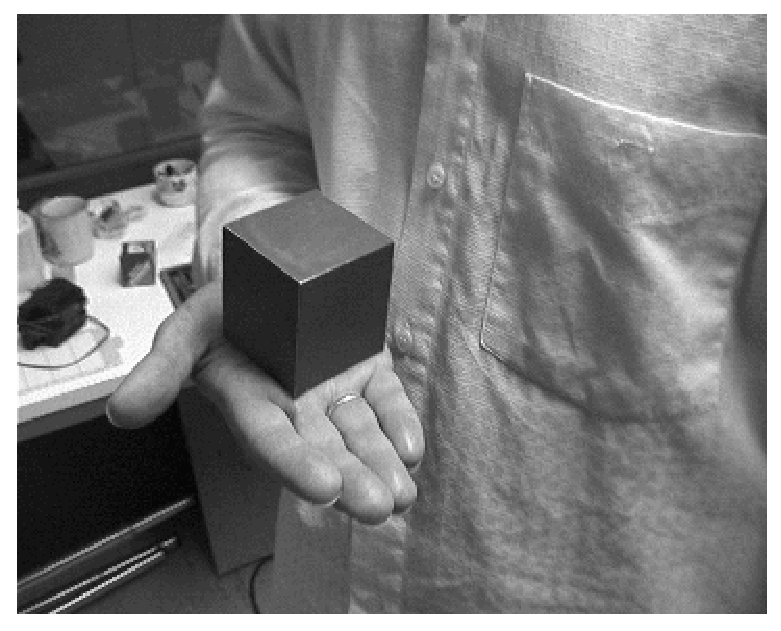
\includegraphics[width=\linewidth]{\figdir/handorig}
		\caption{Originalbild}
		\label{FIG:arexorig}
	\end{subfigure}
	%
	\begin{subfigure}{0.45\linewidth}
		\centering
		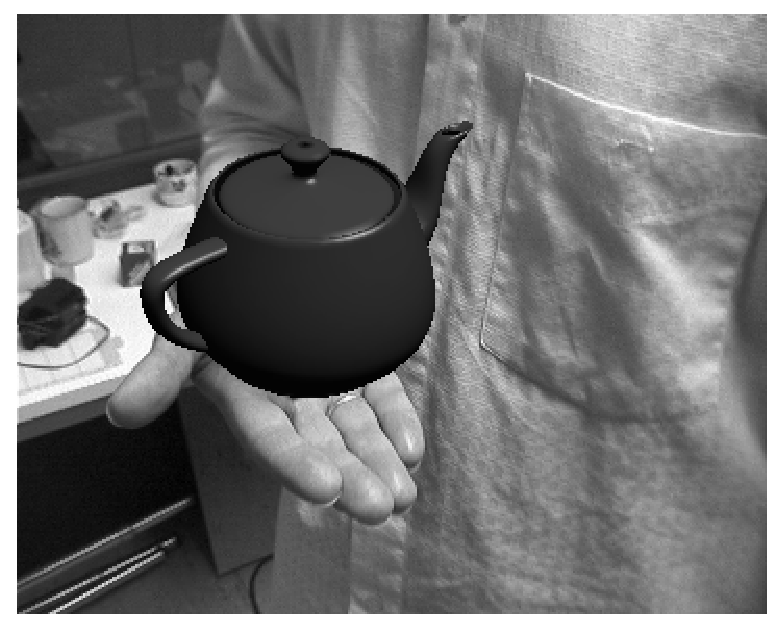
\includegraphics[width=\linewidth]{\figdir/handaug}
		\caption{erweitertes Bild}
		\label{FIG:arexaugm}
	\end{subfigure}
	%
	\caption[AR Beispiel]
	{Beispiel eines Augmented Reality Systems: es folgt eine Beschreibung (Bilder aus \cite{Schmidt01:PAO})}
	\label{FIG:arex}
\end{figure}

Ein Beispiel wird in Abb.\ \ref{FIG:arex} gezeigt.
Das verwendete Objekt ist in Abb.\ \ref{FIG:arexorig} dargestellt, das Ergebnis in Abb.\ \ref{FIG:arexaugm}.

Eine Formel
\begin{equation}
\label{eq:cvp:test}
f(x) = \frac{1}{3} x + 5, \quad x \in \real.
\end{equation}

Und noch eine:
\begin{equation}
\label{eq:cvp:matvec}
\bm{M}  = \bm{Ax} \pi, \quad \bm{A} \in \real^{2 \times 2}, \bm{x} \in \real^2.
\end{equation}

Tabelle \ref{t:CodebookOverview} gibt einen Überblick über XYZ.

\begin{table}[t]
	\centering\small
	%
% generated by TexTableGenerator.pl ((c) Florian Vogt)
% from file: /home/Jochen/data/dissdata/results/CodebookOverview.log
%
\begin{tabular}{l|ccc|cc}
\hline
\hline
                  \textbf{Sequence} &          ARTS &           wman &         stcams &         ARTVZ &        ARTSUZ \\ 
                 \textbf{\# Frames} &             190 &              40 &             400 &             270 &             190 \\ 
     \textbf{\# relative movements} &           17955 &             780 &           79800 &           36315 &           17955 \\ 
\textbf{\# movements after pre-sel.} &           14336 &             623 &           37915 &           21788 &           14343 \\ 
       \textbf{min.\ angle in seq.} &   0.233$^\circ$ &    5.95$^\circ$ &   0.154$^\circ$ & 0.00000171$^\circ$ &  0.0388$^\circ$ \\ 
       \textbf{max.\ angle in seq.} &    81.7$^\circ$ &     180$^\circ$ &    47.3$^\circ$ &    80.3$^\circ$ &    80.9$^\circ$ \\ 
\textbf{min.\ angle after pre-sel.} &    12.9$^\circ$ &    21.1$^\circ$ &    17.3$^\circ$ &    16.3$^\circ$ &    12.9$^\circ$ \\ 
\textbf{max.\ angle after pre-sel.} &    81.7$^\circ$ &     161$^\circ$ &    47.3$^\circ$ &    80.3$^\circ$ &    80.9$^\circ$ \\ \hline\hline
\end{tabular}

	\caption[Testtabelle]{Datenselektion für verschiedene Testdatensätze.}
	\label{t:CodebookOverview}
\end{table}


%%% Local Variables: 
%%% mode: latex
%%% TeX-master: "thesis.tex"
%%% End: 
